% !TeX document-id = {c68f4be8-c497-43e0-82df-e9ebfbea9577}
% !TeX TXS-program:pdflatex = pdflatex -synctex=1 -interaction=nonstopmode --shell-escape %.tex
% новая команда \RNumb для вывода римских цифр
\documentclass[a4paper,12pt]{article}
\usepackage{amssymb}
\usepackage{amsmath}
\usepackage{amsthm} 
\usepackage{caption}
%\usepackage{misccorr}
\usepackage[noadjust]{cite}
\usepackage{cmap} 
\usepackage[utf8]{inputenc}
\usepackage[T2A]{fontenc}
\usepackage[english, russian]{babel}
\usepackage{graphics}
\usepackage{graphicx}
\usepackage{textcomp}
\usepackage{verbatim}
\usepackage{makeidx}
\usepackage{geometry}
\usepackage{float}
\usepackage{bm}
\usepackage{esint}
\usepackage{mathtools}
\usepackage{graphicx}
\usepackage{listings}
\usepackage{courier}
\usepackage{multirow}
\usepackage{graphicx}

\lstset{basicstyle=\fontsize{10}{10}\selectfont,breaklines=true}

\newcommand{\specchapter}[1]{\chapter*{#1}\addcontentsline{toc}{chapter}{#1}}
\newcommand{\specsection}[1]{\section*{#1}\addcontentsline{toc}{section}{#1}}
\newcommand{\specsubsection}[1]{\subsection*{#1}\addcontentsline{toc}{subsection}{#1}}
\newcommand{\RNumb}[1]{\uppercase\expandafter{\romannumeral #1\relax}}
\newcommand{\jj}{\righthyphenmin=20 \justifying}


% геометрия
\geometry{pdftex, left = 2cm, right = 2cm, top = 2.5cm, bottom = 2.5cm}

\setcounter{tocdepth}{4} % фикс переноса 
\righthyphenmin = 2
\tolerance = 2048

\begin{document}
\thispagestyle{empty}

\noindent \begin{minipage}{0.15\textwidth}
	
\includegraphics[width=\linewidth]{b_logo}
\end{minipage}
\noindent\begin{minipage}{0.9\textwidth}\centering
	\textbf{Министерство науки и высшего образования Российской Федерации}\\
	\textbf{Федеральное государственное бюджетное образовательное учреждение высшего образования}\\
	\textbf{«Московский государственный технический университет имени Н.Э.~Баумана}\\
	\textbf{(национальный исследовательский университет)»}\\
	\textbf{(МГТУ им. Н.Э.~Баумана)}
\end{minipage}

\noindent\rule{18cm}{3pt}
\newline\newline
\noindent ФАКУЛЬТЕТ $\underline{\text{«Информатика и системы управления»}}$ \newline\newline
\noindent КАФЕДРА $\underline{\text{«Программное обеспечение ЭВМ и информационные технологии»}}$\newline\newline\newline\newline\newline\newline\newline


\begin{center}
	\noindent\begin{minipage}{1.3\textwidth}\centering
	\Large\textbf{  Лабораторная работа № 5}\newline
	\textbf{по дисциплине "Вычислительные алгоритмы"}\newline\newline\newline
	\end{minipage}
\end{center}

\noindent\textbf{Тема} $\underline{\text{Численное интегрирование.}}$\newline\newline
\noindent\textbf{Студент} $\underline{\text{Романов А.В.}}$\newline\newline
\noindent\textbf{Группа} $\underline{\text{ИУ7-43Б}}$\newline\newline
\noindent\textbf{Оценка (баллы)} $\underline{\text{~~~~~~~~~~~~~~~~~~~~~~~~~~~}}$\newline\newline
\noindent\textbf{Преподаватель} $\underline{\text{Градов В.М.}}$\newline

\begin{center}
	\vfill
	Москва~---~\the\year
~г.
\end{center}
\clearpage
\section{Тема работы}

\noindent Построение и программная реализация алгоритмов численного интегрирования.
\section{Цель работы}

\noindent Получение навыков построения алгоритма вычисления двукратного интеграла с использованием квадратурных формул Гаусса и Симпсона.
\section{Задание}
\noindent Построить алгоритм и программу для вычисления двукратного интеграла при фикчированном значении параметра $\tau$

$$\epsilon (\tau) = \frac{4}{\pi} \int_{0}^{\frac{\pi}{2}} d\phi \int_{0}^{\frac{\pi}{2}} [1 - \exp(-\tau \frac{1}{R})] \; cos\theta \; sin\theta \; d\theta \; d\varphi  $$\newline

\noindent \large{где $ \frac{1}{R} = \frac{2 cos\theta}{1 - cos^2\theta sin^2\varphi}$\newline}

\noindent Применить метод последовательного интегрирования. По одному направлению использовать формулу Гаусса, а по другому -- формулу Симпсона.

\section{Описание алгоритма}
	
\noindent Имеем $\int_{-1}^{1} f(t) dt = \sum_{i = 1}^{n}A_{i}f(t_{i})$, положим $\int_{-1}^{1} t^k dt = \sum_{i = 1}^{n}A_{i}f(t_{i}^k), \; k = 0, 1, 2,..., 2n-1$\newline

\noindent Имеем систему:\newline


$\begin{cases}
	\sum_{i = 1}^{n} A_{i} = 2 \\
	\sum_{i = 1}^{n} A_{i} t_{i} = 0 \\
	\sum_{i = 1}^{n} A_{i} t_{i}^2 = \frac{2}{3} \\
	\dots \\
	\sum_{i = 1}^{n} A_{i} t_{i}^{2n - 1} = 0 \\
\end{cases}$\newline\newline


\noindent Системая нелинейная, найти решение сложно. Для нахождения $A_{i}$ и $t_{i}$ можно воспользоваться полиномом Лежандра. Формула полинома:

$$ P_{n}(x) = \frac{1\;d^n}{2^nn!\;dx^n} [(x^2 - 1)^n], \; n = 0, 1, 2$$

\noindent Узлами формулы Гаусса являются нули полинома Лежандра $P_{n}(t)$, а $A_{i}$ можно найти из вышеуказанной системы уравнений.\newline

\noindent При вычислении интеграла на произвольном интервале $[a, b]$, для применения квадратурной формулы Гаусса необходимо выполнить преобразование переменной:

$$ x = \frac{b + a}{2} + \frac{b - a}{2}t$$

\noindent В таком случае, получаем конечную формулу для произвольного интервала $[a, b]$:

$$ \int_{a}^{b}f(x)dx = \frac{b - a}{2}\sum_{i = 1}^{n} A_{i}f(x_{i})$$

\noindent Так же, существует квадратнурная формула Симпсона:

$$ \int_{a}^{b} f(x)dx \approx \frac{h}{3} \sum_{i = 0}^{\frac{N}{2} - 1} (f_{2i} + 4f_{2i + 1} + f_{2i + 2})$$

\noindent Однако, эти методы можно применять и для приближенной оценки двукратных (и не только) интегралов. Рассмотрим интеграл по прямоугольной области:

$$ I = \int_{c}^{d} \int_{a}^{b} f(x, y)dx\;dy =\int_{a}^{b}F(x)dx, \quad \text{где} \; F(x) = \int_{c}^{d}f(x, y)dy$$\newline


\noindent По каждой координате введем сетку узлов. Каждый однократный интеграл вычисляют по квадратурным формулам. Для разных направлений можно использовать квадратурные формулы разных порядков точности, в т.ч. и Гаусса.\newline

\noindent Конечная формула: 
$$ I = \int\int_{G}f(x, y)dx\;dy = \sum_{i = 1}^{n} \sum_{j = 1}^{m}A_{i}B_{ij}f(x_{i}, y_{j})$$
\noindent \large{где $A_{i}B_{ij}$ -- известные постоянные.}
\clearpage % разрыв страницы

\section{Результаты}
\subsection{Алгоритм вычисления n корней полинома Лежандра n-ой степени.}

\noindent Во-первых, стоит отметить что все корни полинома лежат на интервале [-1, 1]. При этом, интервалы [-1, 0] и [0, 1] -- симметричны, так что при поиске достаточно рассмотреть интервал [0, 1]

\noindent Корни полинома можно вычислить итеративно по методу Ньютона:

$$ x_{i}^{(k + 1)} = x_{i}^k - \frac{P_{n}(x_{i})^{(k)}}{P'_{n}(x_{i})^{(k)}}$$

\noindent причем начальное приближение для $i\text{-го корня}$ берем по формуле:

$$x_{i}^{(0)} = cos[\frac{\pi(4i - 1)}{4n + 2}]$$

\subsection{Влияние количества выбираемых узлов сетки по каждому направлению на точность расчетов.}

\begin{center}
	\begin{tabular}{ | l | l | l | p{1cm} |}
		\hline
		$N$ & $M$ & Результат \\ \hline
		2 & 2 & 0.775 \\ 
		2 & 3 & 0.766 \\ 
		2 & 4 & 0.768 \\ 
		2 & 5 & 0.778 \\ \hline
		3 & 2 & 0.801 \\ 
		4 & 2 & 0.805 \\ 
		5 & 2 & 0.807 \\
		5 & 5 & 0.814 \\				
		\hline
	\end{tabular}
\end{center}

""\newline
\noindent Как можно заметить, при увеличении M (N = 2), результат меньше, чем при равном количестве узлов (N = M = 5). При увеличении N (M = 2) -- видим аналогичную картину, но результат уже ближе к полученному при одинаковом количестве узлов. Таблица составлена при $\tau = 1$.

\subsection{График зависимости $\epsilon(\tau)$.}

\begin{center}
	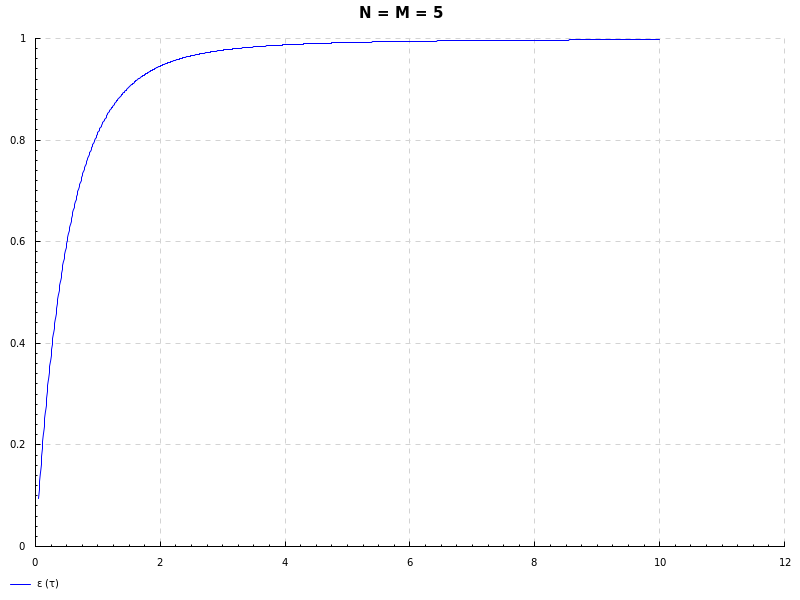
\includegraphics[scale=0.5]{../../src/graph.png} \newline
\end{center}

\noindent Как видно на графике, с увеличением $\tau$ -- увеличивается и $\epsilon(\tau)$, но и не превышает единицы, т.к. $\epsilon(\tau) < 1$.

\section{Ответы контрольные вопросы}
\noindent\textbf{1.} В каких ситуациях теоретический порядок квадратурных формул численного интегрирования не достигается?\newline

\noindent Если подынтегральная функция не имеет соответствующих производных. Например, если на отрезке интегрирования не существует 3-я и 4-я производные, то порядок тончности формула Симпсона будет только 2-ой.\newline


\noindent\textbf{2.} Построить формулу Гаусса численного интегрирования при одном узле.\newline

$$ \int_{a}^{b} = \frac{b - a}{2} \; 2f(\frac{b + a}{2})$$

\noindent $A_{0} = 2, \; t_{0} = 0$

\noindent\textbf{3.} Построить формулу Гаусса численного интегрирования при двух узлах.\newline


$$ \int_{a}^{b} = \frac{b - a}{2} \; (f(\frac{b + a}{2} - \frac{b - a}{2} \frac{1}{\sqrt{3}}) + f(\frac{b + a}{2} + \frac{b - a}{2} \frac{1}{\sqrt{3}})) $$\newline

\noindent $A_{0} = 1, \; A_{1} = 1, \; t_{0} = -\frac{1}{\sqrt{3}}, \; t_{1} = \frac{1}{\sqrt{3}}$ \newline


\noindent\textbf{4.} Получить обобщенную кубатурную формулу, на основе методе трапеций, с тремя узлами на каждом направлении \newline

$$ \int_{c}^{d}\int_{a}^{b}f(x, y)dx\;dy = h_{x} (\frac{1}{2} (F_{0} + F_{2}) + F_{1} ) = $$
$$ = \; h_{x} h_{y} [\frac{1}{4} (f(x_{0}, y_{0}) + f(x_{0}, y_{2}) + f(x_{2}, y_{0}) + f(x_{2}, y_{2})) + $$
$$ + \; \frac{1}{2}(f(x_{0}, y_{1}) + f(x_{2}, y_{1}) + f(x_{1}, y_{0}) + f(x_{1}, y_{2})) + f(x_{1}, y_{1})]$$

\clearpage
\section{Код программы}
\noindent\textbf{Файл Main.hs:}
\lstinputlisting[language=Haskell]{../../src/Main.hs}

\noindent\textbf{\newline Файл Integration.hs:}
\lstinputlisting[language=Haskell]{../../src/Integration.hs}

\end{document}